% TEMPLATE for Usenix papers, specifically to meet requirements of

% https://www.usenix.org/conference/usenixsecurity17/submitting-papers

% Complaints to /dev/null.
% This version uses the latex2e styles, not the very ancient 2.09 stuff.
\documentclass[letterpaper,twocolumn,10pt]{article}
\usepackage{lib/usenix,epsfig,endnotes}
\begin{document}

%don't want date printed
\date{}

%make title bold and 14 pt font (Latex default is non-bold, 16 pt)
\title{\Large \bf 3-Step, 1-Factor Authentication With Custom-Fit, In-Ear EEG}

%for single author (just remove % characters)
\author{
{\rm Your N.\ Here}\\
Your Institution
\and
{\rm Second Name}\\
Second Institution
% copy the following lines to add more authors
% \and
% {\rm Name}\\
%Name Institution
} % end author

\maketitle

% Use the following at camera-ready time to suppress page numbers.
% Comment it out when you first submit the paper for review.
\thispagestyle{empty}


\subsection*{Abstract}
In this paper, we present a system that provides 3-factors of authentication (knowledge, posession and inherence) in a single step, using brain-based authentication via a custom-fit, in-ear EEG. Across all subjects, we achieve a best-case XX\% false acceptance, XX\% false rejection rate with data from only one earpiece. In a preliminary test of an ``imposter'' spoofing attack, we find a 0\% false acceptance rate. \underline{Conclusions and relevance}.

\section{Introduction}
\label{sec:org7196b99}

It is well appreciated by experts and end-users alike that strong authentication is
critical to cybersecurity and privacy, now and into the future. Unfortunately,
news 
reports of celebrity account hackings serve as regular reminders that
the currently dominant method of authentication in consumer applications, 
single-factor authentication using passwords or other user-chosen secrets, 
is faced by many challenges. Major industry players such as Google and
Facebook have been strongly encouraging their users to adopt two-factor
authentication (2FA). However, the need for users to submit two different 
authenticators in two separate steps has frustrated wide adoption, 
due its additional hassle cost to the users. For instance, the popular Apple
iPhone has already implemented the necessary technologies to support device
unlock using either a user-selected passcode or a fingerprint. Therefore the
device could easily support a two-step two-factor authentication scheme if
desired. However, it is easy to understand why users would balk at having to
enter a passcode \emph{and} provide a fingerprint each time they want to unlock their phone.

In previous work, “one-step two-factor authentication” has been proposed as a
new approach to authentication that can provide the security benefits of two-
factor authentication without incurring the hassle costs of two-step verification.
By employing consumer-grade EEG (electroencephalogram) sensing
technologies, it was demonstrated in a 2013 passthoughts study that a user can
submit both a knowledge factor (i.e., secret thought) and an inherence factor
(i.e., brainwave signal unique to the individual) in a single step by performing a
single mental task. Additionally, the robustness of this method against
impersonation attacks was demonstrated, including conditions where the attacker
may have learned the target’s secret thought and/or secret task.

In the present proposal, we will undertake, to the best of our knowledge, the first
ever study of one-step three-factor authentication. In computer security,
authenticators are classified into three types: knowledge factors (e.g., passwords
and PINs), possession factors (e.g., physical tokens, ATM cards), and inherence
factors (e.g., fingerprints and other biometrics). Because three-factor
authentication (3FA) requires the user to submit one distinct instance of each
type of authenticator, it represents the strongest level of authentication security
possible.

We propose the use of custom-fit Ear EEG technology as the platform for
investigating the feasibility, performance, and usability of one-step three-factor
authentication. In addition to the same knowledge factor and inherence factor as
in previous work, the user can submit in the same step the possession factor
in the form of the EEG-sensing ear-piece(s) that are custom-fitted to and worn in
their ear. These earpieces can serve as physical tokens in the same way as bank
ATM cards and wearable hardware tokens. Furthermore, because the earpieces
are custom-fitted to each individual, they will likely not be able to produce good
electrical impedances when worn by a different individual.

\section{Related work}
\label{sec:org3732d7c}

The use of EEG as a biometric signal for user authentication has a short history.
In 2005, Thorpe et al. motivate and outline the design of a passthoughts system,
where, rather than typing a password, users authenticate 
by thinking of a passthought. Since 2002, a number of independent groups have achieved 99-
100$\backslash$% authentication accuracy using multi-channel sensors placed on the scalp. In 2013, one group showed that 99$\backslash$% authentication accuracy can also be
achieved using a consumer-grade single-channel sensor. In particular, the
lack of signal diversity from multiple EEG channels can be overcome by allowing
the users to choose their own personalized passthoughts (e.g., sing their favorite
song in their head). There are two significant consequences of this result. First,
the passthoughts approach is no longer constrained by the high cost (> \$10,000 USD)
and low usability (gel-based electrodes; aesthetic challenges of an EEG cap) of
medical-grade multi-channel devices. Second, because users can choose and
easily change their secret mental task, this approach can support one-step two-
factor authentication via the simultaneous presentation of the inherence factor
(brainwave signatures due to the unique folding structures of the cortex) and the
knowledge factor (the secret mental task).

\begin{figure}[htbp]
\centering
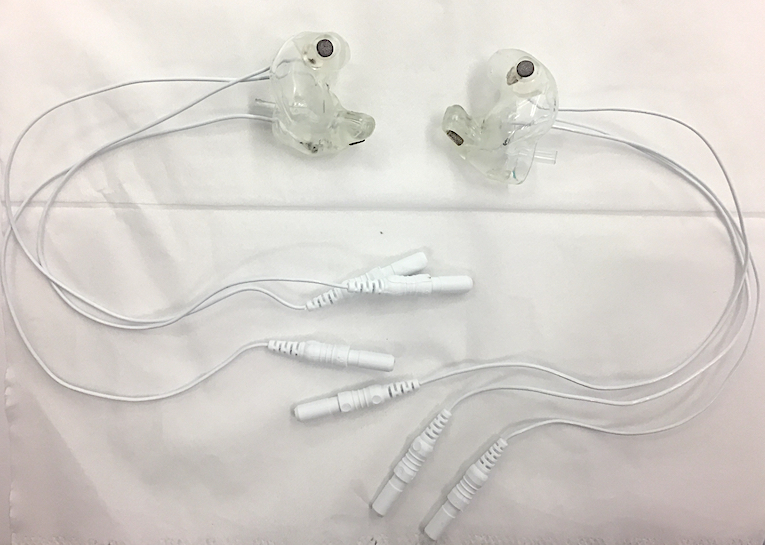
\includegraphics[width=.9\linewidth]{./figures/2EEEG.jpg}
\caption{Pair of custom-fit earpieces with 3 embedded electrodes each located at the helix and front-facing and back-facing within the ear canal.}
\end{figure}

Research in in-ear EEG is only several years old. Nonetheless, the concept has
attracted a lot of attention because of the discreetness factor of in-ear EEG over
traditional scalp-based EEG. A research team at the Imperial College London
and Aarhus University published a landmark paper in 2011 that introduced the
concept of in-ear EEG, demonstrating for the first time the feasibility of recording
brainwave signals from within the ear canal. Follow-up work from the same
group demonstrated its ability to produce signal-to-noise ratios comparable to
those from conventional EEG electrode placements, robustness to common
sources of artifacts, and use in a brain-computer interface (BCI) system based on
auditory evoked potentials and visual evoked potentials.
\underline{Citation to our past work} 
was the first to merge these two streams of work, using in-ear EEG signals for
user authentication with a consumer-grade device. United Sciences is currently
developing a consumer hearable called The Aware that will measure EEG from the ear.
Behavioral authentication methods such as keystroke dynamics and speaker
authentication can be categorized as one-step two-factor authentication
schemes. In both cases, the knowledge factor (password or passphrase) and
inherence factor (typing rhythm or speaker’s voice) are employed. In contrast, the
Nymi band supports one-step two-factor authentication via the inherence
factor (cardiac rhythm that is supposed to be unique to each individual) and the
possession factor (the wearing of the band on the wrist). However, as far as we
know, no one has proposed or demonstrated a one-step three-factor
authentication scheme.
\section{Methods}
\label{sec:org63d105c}
\subsection{{\bfseries\sffamily TODO} Manufacturing, materials}
\label{sec:orgb483219}
\subsection{Subjects}
\label{sec:orgaf30da9}
\subsection{{\bfseries\sffamily TODO} Tasks}
\label{sec:org86eea32}

\underline{Explain stuff around tasks}

\begin{table}[h]
\centering
\begin{tabular}{ll}
\textbf{\textbf{Task}} & \textbf{\textbf{Description}}\\
\hline
Breathe & Relaxed breathing with eyes closed.\\
Breathe - Open & Relaxed breathing with eyes open.\\
Sport & Sport-related motor imagery of participant's choice.\\
Song & Imagining a song of participant's choice playing.\\
Song - Open & Imagining a song with eyes open.\\
Speech & Imagining a phrase of participant's choice being spoken.\\
Listen & Tone \& Listening to a continuous tone.\\
Listen - ASSR & Listening to noise modulated at 40 Hz.\\
Face & Imagining a person's face of participant's choice.\\
Sequence & On timed cues, imagine a face, a number, and a word.\\
\hline
\end{tabular}
\caption{Set of tasks proposed for authentication with descriptions.}
\end{table}

\begin{table}[h]
\centering
\begin{tabular}{lllll}
Task & External stimuli? & Knowledge factor ? & Eyes? & Imagery?\\
\hline
Breathe & No & No & Closed & None\\
Breathe - open & No & No & Open & None\\
Sport & No & Yes & Closed & Motor\\
Song & No & Yes & Closed & Aural\\
Song - open & No & Yes & Open & Aural\\
Speech & No & Yes & Closed & Aural\\
Listen - Tone & Yes & No & Closed & None\\
Listen - ASSR & Yes & No & Closed & None\\
Face & No & Yes & Closed & Visual\\
Sequence & Yes & Yes & Open & Visual\\
\hline
\end{tabular}
\caption{Properties of authentication tasks. We selected tasks with a variety of different properteries, but preferred tasks that did not require external stimuli, as the need to present such stimuli at authentication time could present challenges for usability, and user security.}
\end{table}
\subsection{Protocol}
\label{sec:org2041857}
Our initial participants were recruited from a nearby university and scheduled for ear molding
and impedance checking sessions. Finally, the data collection visit was scheduled and took
approximately 90 minutes for set up and experiment execution. The OpenBCI system we used
allows for 8 channels of simultaneous recording, along with separate ground and reference channels.
Data was initially collected with the ground placed at the center of the forehead, and using the left
mastoid as reference, though we can easily re-reference to another channel by subtracting a desired
channel (such as right mastoid). Each earpiece (shown in the image below) contain three channels: 
one placed on the helix, and two inside the canal - one front-facing and the other back-facing. The remaining
two channels were placed on the right mastoid for later re-referencing, and at approximately Fp1 (on the 
forehead above the left eye) for validating the data collected in the ears against a scalp-based measure. 
Before beginning the experiment, the data from all channels was visualized and participants were asked to
blink and clench their jaws to confirm visibly that all channels were active and properly connected.

During the experiment, participants were seated in a comfortable position in a quiet room facing a laptop screen on which the
instructions and stimuli were presented using PsychoPy. Each task was completed once in sets five trials each, and then
each was completed again for another five trials. Each trial was 10 seconds in length, for a total of 10 trials and 
100 seconds of data collected per task. The instructions were read aloud to the participant by the experimenter, and
the experiment was advanced using a pointer held in the participant's lap to minimize motion artifacts in the data.  
The experimenter also recorded the participant's chosen secrets for the sport, song, face, speech, and sequence
 tasks and reminded the participant of these for the second set of trials.
\section{Analysis}
\label{sec:org6c1a839}
\subsection{Validating the data}
\label{sec:org800f2bd}

In this section, we establish that the data we collected were EEG signals with relatively low noise. 
Using the pilot data from two participants, we were able to confirm the custom-fit earpieces are able to collect EEG
data using three tests: good impedances measured for the ear electrodes, alpha-band activity attenuation when a
participant's eyes were open versus closed, and the presence of a significant ASSR signal.

The recorded impedances of the earpiece electrodes were less than 5 kOhms except one, a benchmark used widely in previous
ear EEG work. The left helix electrode of one participant was measured at 9 kOhms, and generally the 
helix impedances for both participants were higher than their ear canal counterparts. We expected this result, given that the
helix electrode relies on quality of the earpiece's fit outside the ear for good contact, and is not as securely and tightly placed as the
electrodes within the ear canal. Nonetheless, the data from all electrodes were tested in the remaining two data quality tests.

For the alpha-attenuation test, data from the "Breathe" task was compared with that of the "Breathe - Open" task. It is a well-
known feature of EEG data that activity in the alpha-band (approximately 8-12 Hz range) increases when the eyes are closed
compared with a similar state with eyes open. For both of our pilot participants this attenuation is clearly visible even in just
a single trial's data. To further validate, we also performed this calculation on the data collected from the Fp1 electrode and see
the effect clearly here as well. It is important to note that the left ear results are reported using the right mastoid as reference, and
the right ear results in turn using the left mastoid as reference. When using the same side mastoid for reference the effect is not 
visible, though it may be if we average across many trials. This is not surprising, as the further a reference electrode is from the active
channel the less "real" signal is being subtracted from the active channel. This has important design implications for eventual 
real-world deployment of this authentication method however, as it will likely require pieces worn on or around both ears to properly 
function, and not just one. The figures below show the alpha attenuation in the left and right ear channels, as well as Fp1.

\begin{figure}[h]
\centering
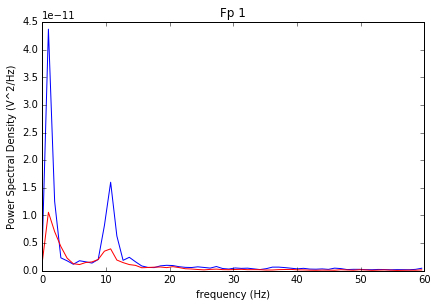
\includegraphics[width=0.5\textwidth]{figures/001_AlphaAtt_Fp1.jpg}
\caption{Alpha-attenuation (8-12 Hz range) in Fp1 channel, referenced at left mastoid, for comparison to ear channels. Red indicates breathing data with
eyes open, blue indicates the same task with eyes closed.}
\end{figure}

\begin{figure}[h]
  \centering
  \begin{minipage}[b]{0.45\textwidth}
    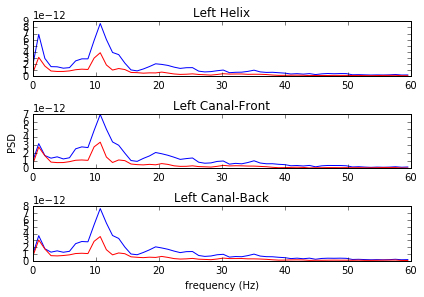
\includegraphics[width=\textwidth]{figures/001_AlphaAtt_Left.jpg}
  \end{minipage}
  \hfill
  \begin{minipage}[b]{0.45\textwidth}
    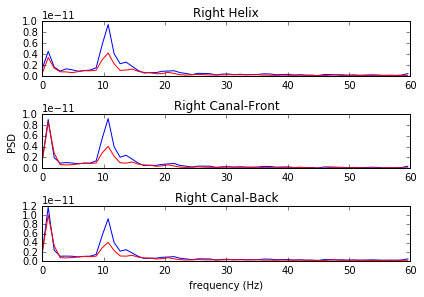
\includegraphics[width=\textwidth]{figures/001_AlphaAtt_Right.jpg}
  \end{minipage}
\caption{Alpha-attenuation (8-12 Hz range) in left and right ear canal channels, referenced at opposite mastoids respectfully. Red indicates breathing data with
eyes open, blue indicates the same task with eyes closed.}
\end{figure}

Finally, for the ASSR test we calculated power spectra for data from the "Listen - ASSR" task. The audio stimulus used for this task is modulated 
at 40 Hz, which should, in turn, produce an EEG response visible in the data at 40 Hz. Strangely, in our tests we do see an ASSR spike but it is located 
around 74 Hz instead. While this has us somewhat perplexed about our stimulus, the purpose of this test was to ensure that the response seen in the ear channels 
matched the response seen from the Fp1 recordings, which is evident comparing the figures below.

\begin{figure}[h]
\centering
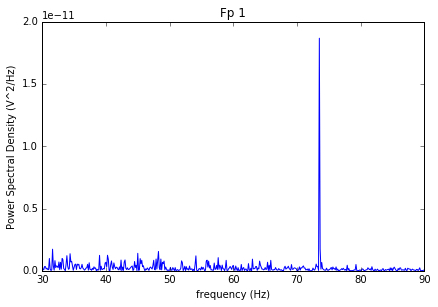
\includegraphics[width=0.5\textwidth]{figures/001_ASSR_Fp1.jpg}
\caption{Power spectrum for data collected from the Fp1 channel during 40 Hz ASSR stimulus. An ASSR spike is clearly visible, though not at 40 Hz where it was expected.}
\end{figure}

\begin{figure}[h]
  \centering
  \begin{minipage}[b]{0.45\textwidth}
    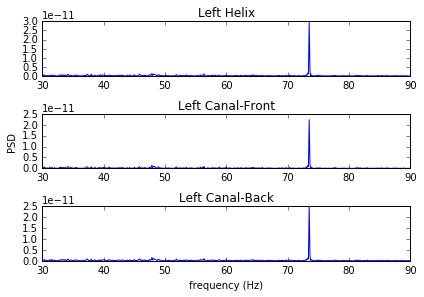
\includegraphics[width=\textwidth]{figures/001_ASSR_Left.jpg}
  \end{minipage}
  \hfill
  \begin{minipage}[b]{0.45\textwidth}
    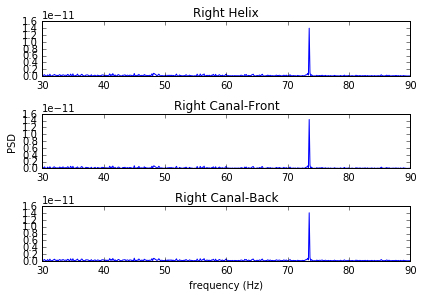
\includegraphics[width=\textwidth]{figures/001_ASSR_Right.jpg}
  \end{minipage}
\caption{Power spectra for data collected from the earpiece channels during 40 Hz ASSR stimulus. Again, the spike is clearly visible though not at 40 Hz, however it 
does match the activity measured at Fp1.}
\end{figure}

\subsection{Classification}

We analyzed the EEG signals collected during the tasks using a support vector classifier (SVC). Since past work has shown that classification tasks in EEG-based BCI are linear \underline{cite}, we used XGBoost, a popular tool for generating ensemble classifiers for logistic linear classification \underline{cite}.

To produce feature vectors, we took slices of 100 raw values from each electrode (about 500ms of data), and performed an FFT to produce power spectra for each electrode during that slice. We concatenated all electrode power spectra together, and performed PCA on all concatenated vectors such that the resulting vectors described 95\% of the variance in the full power specrum data. For each task, for each participant, 100 seconds of data were collected in total across 10 trials of 10 seconds each, resulting in 200 samples per participant, per task, following preprocessing.

We trained the classifier using a balanced sample of positive and negative examples, where positive examples were from the target subject and target task, and negative examples were randomly selected tasks from any subject besides the target subject.
From this corpus of positive and negative samples, we withheld one third of data for testing. 
The remaining training set was fed into a XGBoost's cross-validation method, which we set to iteratively tweak parameters over a maximum of fifty rounds of cross-validation to minimize classification error.
After cross-validation, the updated classifier (with paramters applied) predicted labels on each sample in the test set, and we calculated FAR and FRR on its results.

\subsection{{\bfseries\sffamily TODO} Simulating an imposter attack}
\label{sec:orgdd6e8bd}
\section{Results}
\label{sec:org6705b1d}
\subsection{{\bfseries\sffamily TODO} Combinations of electrodes}
\label{sec:org21b14ae}

\underline{Figure: Plot of FAR/FRR by electrode combination, XGBoost and LinearSVC}.

\subsection{{\bfseries\sffamily TODO} Left-ear authentication}
\label{sec:org82cbcf4}

\underline{Our main result:}

\underline{Table: FAR/FRR Between-subjects results by participant (avg. all tasks? Best task?)}

\underline{Our attempt to substantiate that we have both inherence and knowledge factors:}

\underline{Table: original strategy, within-subjects, within-tasks strategy; where each of those headings is subdivided into mean FAR, mean FRR (across all subjects and tasks)}

\subsection{Imposter attack}

While our left-ear results establish that passthoughts achieve low FAR and FRR when tested against other subjects' passthoughts, we do not know how robust passthoughts are against a spoofing attack, in which both a subject's custom-fit electrode, and details of that subject's chosen passthought, are leaked. 

To explore this scenario, we chose one subject (subject 6), and referred to their report of chosen passsthoughts. We recorded spoofed passthoughts for two ``imposter'' subjects. One subject appeared in our initial pool performing their own passthoughts (subject 2), while the other subject did not appear in the initial pool, and thus was not included when training subject classifiers. (How well the imposters were able to spoof subject 6's passthought is an open question; see Discussion).

For each task, we ran the spoofed version of the task through the classifier trained on subject 6's task as the passthought.
None of the spoofed passthoughts were accepted, resulting in a 0\% FAR.


\subsection{{\bfseries\sffamily TODO} Usability}
\label{sec:org18d5968}

\underline{Quantitative and qualitative data, where appropriate}

\section{Discussion}

Our findings demonstrate the apparent feasibility of single earpiece, achieving good results with only three electrodes and a reference, all on the left ear. FARs and FRRs are low across all subjects and tasks, with FARs overall lower than FRRs. Subjects' best-performing passthoughts typically seeing no errors in our training. Furthermore, no spoofed attacks were successful in our cursory analysis.

The powerful interactions between inherence and knowledge emerged in our spoofing attack. Although our target subject documented their chosen passthought, the spoofers found ambiguity in how these passthoughts could be expressed. For the face task, the spoofers did not know the friend the original subject had chosen. For the song tasks, though the song was known, the spoofers did not know what part of the song the original subject had imagined, or how it was imagined (humming, imagining a full performance, melody, vocals, etc). This experience sheds light on the highly individual nature of passthoughts, and provides a positive indication that there may be some intrinsic difficulty ofr spoofing passthoughts.

In our analysis, some notable patterns emerged. First, \textit{breathe} tended to be the best-performing task among participants. Classifiers overall distinguished the breath task even compared to breath tasks from other subjects, implying that the task is expressed differently for each subject, i.e. that this task has an inherence factor sufficient for authentication, even though the task does not have a knowledge factor. Second, we were able to achieve good results by generating feature vectors based on only 500ms (300 voltage readings across the three electrodes). This short timespan is somewhat surprising, given that some tasks (like songs) presumably rely on changes or patterns over a longer period of time. 

Counter to our expectations, we found that referencing on the same side as the electrodes improves classification accuracy, compared to referencing on the other side of the head, as is commonly done in EEG. \underline{Theory as to why?} Furthermore, the use of conductive gel results in decent results (low impedances) on other subjects' custom-fit earpieces. This is somewhat surprising, since ear canals are believed to be more unique than fingerprints \underline{cite}. Finally, performance on FP1 was not as high as performance in the ear, despite FP1's popularity in past work on passthoughts \underline{cite}. This could be explained by the greater number of electrodes in the ear (compared to just one on FP1). Another explanation might be in the neural activity required to perform the tasks we chose. Future work might shed light on this issue.


\section{Future Work}

One primary question surrounds how our passthought system performance will change with a greater number of users, and with more diverse data. Our system specifically trains on negative examples of non-users; we do not yet know how this approach will scale. At the same time, we must investigate the stability of EEG readings for a passthought are over time. We must also collect EEG data from the variety of different user states: ambulatory settings, during physical exertion or exercise, under the influence of caffeine or alcohol, etc.

% We provide cursory evidence that passthoughts are difficult to spoof, though further work should expand on ours with more subjects.
Another important question surrounds how passthoughts might be cracked.
Generally, we do not understand how an individual's passthought is drawn from the general distribution of EEG signals that an individual produces throughout the day.
Given a large enough corpus of EEG data, are some passthoughts as easy to guess as \textit{password1234} is for passwords?
Future work should perform statistical analysis on passthoughts, such as clustering (perhaps with t-SNE) to better understand the space of possible passthoughts.
This work will allow us simulate cracking attempts, and to develop empirically motivated strategies for prevention, e.g. locking users out after a certain number of attempts.
This work could also reveal interesting tradeoffs between the usability and accuracy of certain passthoughts with their security properties.

Finally, our work leaves room for some clear UX improvements.
Future work should try using dry electrodes, commonly found in consumer EEG devices, for comfort and usability.
Future work should also attempt a closed-loop (or online) passthought system, in which users receive immediate feedback on the result of their authentication attempt. A closed-loop BCI system could help us understand how learning effects
on the human side might impact authentication performance, as the human and machine co-adapt during multiple authentication attempts.

\section{TODO Conclusion}

\end{document}
